%% 该模板修改自《计算机学报》latex 模板
%% 主要是将双栏改成单栏，去掉了部分计算机学报标识；
%% 源文件自：https://www.overleaf.com/latex/templates/latextemplet-cjc-xelatex/ybmmymncrrmw
%% 
%%
%% This is file `CjC_template_tex.tex',
%% is modified by Zhi Wang (zhiwang@ieee.org) based on the template 
%% provided by Chinese Journal of Computers (http://cjc.ict.ac.cn/).
%%
%% This version is capable with Overleaf (XeLaTeX).
%%
%% Update date: 2026/09/10
%% -------------------------------------------------------------------
%% Copyright (C) 2016--2026 
%% -------------------------------------------------------------------
%% This file may be distributed and/or modified under the
%% conditions of the LaTeX Project Public License, either version 1.3c
%% of this license or (at your option) any later version.
%% The latest version of this license is in
%%    https://www.latex-project.org/lppl.txt
%% and version 1.3c or later is part of all distributions of LaTeX
%% version 2008 or later.
%% -------------------------------------------------------------------

\documentclass[10.5pt,compsoc,UTF8]{CjC}
\usepackage{ctex}
\usepackage{graphicx}
\usepackage{footmisc}
\usepackage{subfigure}
\usepackage{url}
\usepackage{multirow}
\usepackage{multicol}
% The gbt7714 package already loads natbib; avoid a cite/natbib conflict.
\usepackage{amsmath,amsthm}
\usepackage{amssymb,amsfonts}
\usepackage{booktabs}
\usepackage{color}
\usepackage{ccaption}
\usepackage{booktabs}
\usepackage{float}
\usepackage{fancyhdr}
\usepackage{caption}
\usepackage{xcolor,stfloats}
\usepackage{comment}
\setcounter{page}{1}
\graphicspath{{figures/}}
\usepackage{cuted}%flushend,
\usepackage{captionhack}
% Figures are PDF files; no EPS conversion is needed for XeLaTeX.
\usepackage{gbt7714}
\usepackage{longtable}
\usepackage{fvextra}
\setmonofont{DejaVu Sans Mono}
\setCJKmonofont{FandolFang-Regular.otf}
\usepackage{array}
\newcommand{\added}[1]{\textcolor{black}{#1}}
\newcommand{\redcite}[1]{{\color{black}\cite{#1}}}
\setlength{\emergencystretch}{1em}
\setlength{\headheight}{26pt}


%===============================%

\headevenname{\mbox{\quad} \hfill  \mbox{\zihao{-5}{ \hfill 数字图像处理  } \hspace {50mm} \mbox{2026 年 10 月}}}%
\headoddname{李建辉，苏威贤，王妍，李定一 \hfill 低剂量 CT 图像的传统去噪与插值增强方法对比研究 }%

%footnote use of *
\renewcommand{\thefootnote}{\fnsymbol{footnote}}
\setcounter{footnote}{0}
\renewcommand\footnotelayout{\zihao{5-}}

\newtheoremstyle{mystyle}{0pt}{0pt}{\normalfont}{1em}{\bf}{}{1em}{}
\theoremstyle{mystyle}
\renewcommand\figurename{figure~}
\renewcommand{\thesubfigure}{(\alph{subfigure})}
\newcommand{\upcite}[1]{\textsuperscript{\cite{#1}}}
\renewcommand{\labelenumi}{(\arabic{enumi})}
\newcommand{\tabincell}[2]{\begin{tabular}{@{}#1@{}}#2\end{tabular}}
\newcommand{\abc}{\color{white}\vrule width 2pt}
\renewcommand{\bibsection}{}
\makeatletter
\renewcommand{\@biblabel}[1]{[#1]\hfill}
\makeatother
\setlength\parindent{2em}
%\renewcommand{\hth}{\begin{CJK*}{UTF8}{gbsn}}
%\renewcommand{\htss}{\begin{CJK*}{UTF8}{gbsn}}


\begin{document}

\hyphenpenalty=50000
\makeatletter
\newcommand\mysmall{\@setfontsize\mysmall{7}{9.5}}
\newenvironment{tablehere}
  {\def\@captype{table}}

\let\temp\footnote
\renewcommand \footnote[1]{\temp{\zihao{-5}#1}}


\thispagestyle{plain}%
\thispagestyle{empty}%
\pagestyle{CjCheadings}

% \begin{table*}[!t]
\vspace {-13mm}


\onecolumn
\zihao{5-}\noindent 李建辉，苏威贤，王妍，李定一 \hfill DIP \& 低剂量 CT 图像的传统去噪与插值增强方法对比研究 \hfill 2026 年 10 月\\
\noindent\rule[0.25\baselineskip]{\textwidth}{1pt}

% \onecolumn
% \zihao{5-}\noindent 第??卷\quad 第?期 \hfill 计\quad 算\quad 机\quad 学\quad 报\hfill Vol. ??  No. ?\\
% \zihao{5-}
% 20??年?月 \hfill CHINESE JOURNAL OF COMPUTERS \hfill ???. 20??\\ 
% \noindent\rule[0.25\baselineskip]{\textwidth}{1pt}

{
\centering
\vspace {11mm}
{\zihao{2} \heiti 低剂量 CT 图像的传统去噪\\与插值增强方法对比研究 }
%题目（中英文题目一致) 字体为 2 号黑体 (全文除特别声明外，外文统一用 Times New Roman)
\vskip 5mm

{\zihao{4}\fangsong 李建辉\quad  苏威贤 \quad 王妍 \quad 李定一}
%字体为 3 号仿宋 * 作者
% \footnote{\noindent \zihao{6} 
% % 收稿日期：\quad \quad -\quad -\quad ；最终修改稿收到日期：\quad \quad -\quad -\quad .*投稿时不填写此项*. 本课题得到… …基金中文完整名称(No.项目号)、… …基金中文完整名称(No.项目号)、… … 基金中文完整名称(No.项目号)资助.
% \textsf{作者名1}，学号，学位(或目前学历),主要研究领域为*****、****. E-mail: **************.\textsf{作者名2}，学号，学位(或目前学历),主要研究领域为*****、****. E-mail: **************. \textsf{作者名3}，学号，学位(或目前学历),主要研究领域为*****、****. E-mail: **************.}

\vspace {5mm}
% \zihao{6}{\textsf{论文定稿后，作者署名、单位无特殊情况不能变更。若变更，须提交签章申请，国家为中国可以不写，省会城市不写省名，其他国家必须写国家名。}}
}

\vskip 5mm
%%%%%%%%%%%%%%%%%%%%%%%%%%摘要%%%%%%%%%%%%%%%%%%%%%%%%%%%%%
\zihao{5}{
\setlength{\baselineskip}{16pt}\selectfont{
\noindent {\heiti 摘\quad 要\quad }
针对低剂量 CT（Low-Dose CT，LDCT）图像噪声较强、细节退化等问题，
本文采用传统数字图像处理方法进行去噪与超分辨率重建。
实验比较均值、高斯、自适应中值、非局部均值（Non-Local Means，NLM）和小波软阈值五种去噪方法，
定量分析结果表明，在本实验设置下，NLM 综合表现最佳，峰值信噪比（PSNR）和结构相似性（SSIM）分别为 39.252 dB 和 0.95269，
较原始 LDCT 分别提高 2.368 dB 和 0.04353。
进一步以 NLM 去噪结果构造低分辨率输入，
比较最近邻、双线性和双三次三种 4 倍插值方法，
结果表明双三次插值取得最高 PSNR 28.005 dB 和 SSIM 0.88673。
顺序实验表明，先去噪后超分优于先超分后去噪。
综合实验结果，本文推荐采用“先 NLM 去噪、后双三次插值”的处理流程。
\par}}
\vspace {5mm}

\zihao{5}{\noindent
{\heiti 关键词 \quad }低剂量 CT；图像去噪；非局部均值；超分辨率重建；双三次插值；结构相似性
}
% \zihao{5-}{\heiti 中图法分类号\quad } TP\rm{\quad \quad \quad     }
% {\heiti DOI号:\quad } *投稿时不提供DOI号


\vskip 7mm

% \begin{center}
% \zihao{3}{ \heiti Title *（中英文题目一致)字体为4号Times New Roman,加粗* Title}\\
% \vspace {5mm}
% \zihao{5}{ NAME Name-Name$^{1)}$ NAME Name$^{2)}$ NAME Name-Name$^{3)}$ *字体为5号Times new Roman*Name}\\
% \vspace {2mm}
% \zihao{5-}{{$^{1)}$(Department of ****, University, City ZipCode, China) *字体为小5号Times new Roman* Depart.Correspond}}

% \zihao{5-}{{$^{2)}$(Department of ****, University, City ZipCode)*中国不写国家名*}}

% \zihao{5-}{{$^{3)}$(Department of ****, University, City ZipCode, country)*外国写国家名*}}

% \end{center}
%%%%%%%%%%%%%%%%%%%%英文摘要%%%%%%%%%%%%%%%%%%%%%%%%%%%%%
\zihao{5}{
\setlength{\baselineskip}{18pt}\selectfont{
{\bf Abstract}\quad \hyphenpenalty=500\relax 
\zihao{5}{\ To address the problems of strong noise and detail degradation in low-dose computed tomography (LDCT) images, this study employs traditional digital image processing methods for denoising and super-resolution reconstruction. Five denoising methods, including mean filtering, Gaussian filtering, adaptive median filtering, Non-Local Means (NLM), and wavelet soft-thresholding, are compared. Quantitative results show that, under the experimental settings of this study, NLM achieves the best overall performance, with a peak signal-to-noise ratio (PSNR) of 39.252 dB and a structural similarity index (SSIM) of 0.95269, representing improvements of 2.368 dB and 0.04353, respectively, over the original LDCT image. Furthermore, low-resolution inputs are constructed from the NLM-denoised results, and three 4× interpolation methods, namely nearest-neighbor, bilinear, and bicubic interpolation, are compared. The results show that bicubic interpolation achieves the highest PSNR of 28.005 dB and SSIM of 0.88673. The processing-order experiment further shows that denoising before super-resolution performs better than super-resolution before denoising. Based on the overall experimental results, the processing pipeline of “NLM denoising followed by bicubic interpolation” is recommended under the experimental conditions of this study. %Do not modify the amount of space before and after the artworks. One- or two-column format artworks are preferred. All Schemes, Equations, Figures, and Tables should be mentioned in the text consecutively and numbered with Arabic numerals, and appear below where they are mentioned for the first time in the main text.
\par}}
\vspace {5mm}

{{\bf Keywords}\quad 
low-dose computed tomography; image denoising; Non-Local Means; super-resolution reconstruction; bicubic interpolation; structural similarity}}



%%%%%%%%%%%%%%%%%%%%%%%%%%%%%%%%%%%%%%
\zihao{5}
\vskip 10mm
% \begin{multicols}{1}


%%%%%%%%%%%%%%%%%%%%%%%%%%%%%%%%%%%%%%%%%%%%%%%%%%%%%%%%%%%%%%%%%%%%%%%
%%%%%%%%%%%%%%%%%%%%%%%%%%%%%%%%%%%%%%%%%%%%%%%%%%%%%%%%%%%%%%%%%%%%%%
%%%%%%%%%%%%%%正文%%%%%%%%%%%%%%%%%%%%%%%%%%%%%%%
\section{\heiti 引言}
%介绍低剂量 CT 的噪声问题、去噪与细节保留的矛盾，以及本实验的目标和主要工作。
低剂量CT通过降低管电流或缩短曝光时间减少辐射剂量，但光子数不足会引入强烈的泊松噪声、条状伪影和颗粒感\redcite{yu2009dose}，同时受成像系统空间分辨率限制，肺小结节、细小支气管和末梢血管的边缘容易模糊。但去噪与细节保留之间存在天然矛盾：平滑滤波能抑制噪声，却会模糊边缘和细小结构；保边滤波能保留结构，却可能残留噪声或产生伪影。传统插值超分也只能基于已有像素估计新像素，无法恢复采集或降采样过程中已经丢失的真实高频信息\redcite{gonzalez2018digital,keys1981cubic}。我们的目标是在完全不使用神经网络的前提下，利用传统图像处理方法对低剂量CT进行噪声抑制和4倍超分辨率增强，并以严格配对的全剂量CT为参考，评价不同去噪与插值组合的效果。我们读取配对DICOM切片并进行肺窗预处理；比较均值滤波、高斯滤波、自适应中值滤波、非局部均值滤波和小波软阈值去噪；选取代表性去噪结果进行最近邻、双线性和双三次插值放大；以全剂量CT为真值，结合主观视觉和PSNR、SSIM指标评价重建质量，并分析去噪与超分的先后顺序对最终结果的影响。
\section{\heiti 相关工作}
%2.1 传统空间域去噪；2.2 小波域去噪；2.3 图像插值增强。简要比较各类方法的特点，为后续方法选择作铺垫。
\subsection{传统空间域去噪}
空间域去噪直接对像素邻域进行运算。均值滤波以邻域均值替代中心像素，计算简单，但会模糊边缘和细小结构。高斯滤波使用高斯核加权，平滑效果比均值滤波自然，但核尺寸和标准差增大时仍会损失细节\redcite{gonzalez2018digital}。中值滤波对脉冲噪声有较好抑制作用，但普通中值滤波对CT颗粒噪声和低对比结构保持能力有限。自适应中值滤波根据局部窗口内灰度分布动态调整窗口大小，在抑制噪声的同时尽量保护边缘\redcite{hwang1995adaptive}。非局部均值滤波利用图像中重复纹理和自相似结构，通过图像块相似度加权平均来估计像素，\added{利用非局部自相似信息兼顾噪声抑制与结构保持}，但计算量较大，滤波参数对结果影响明显\redcite{buades2005nlm}。总体而言，空间域方法实现简单、易于控制，但线性平滑容易模糊细节，非线性方法在噪声抑制和结构保持之间各有取舍。
\subsection{小波域去噪}
小波变换将图像分解为低频近似和不同方向、不同尺度的高频细节。低剂量CT随机噪声多集中在高频子带，因此可对高频系数进行阈值收缩。软阈值函数为\redcite{donoho1995denoising}
\[
T_{\lambda}(x)=\mathrm{sgn}(x)\max(|x|-\lambda,0)
\]
其中\added{\(\lambda\)}为阈值。阈值过大时会丢失细小结节和血管边缘，阈值过小时噪声残留明显。与小波相比，空间域方法直接在像素上操作，计算更简单，\added{小波域方法提供多尺度表示，但噪声和真实结构均可能包含高频成分，其效果取决于阈值和图像特征，不能仅凭变换域表示保证医学图像细节得到更好保留。}本实验选择小波软阈值作为变换域去噪的代表方法。
\subsection{图像插值增强}
传统超分辨率插值根据低分辨率图像中已有像素的灰度连续性估计高分辨率网格上的像素值\redcite{gonzalez2018digital}。最近邻插值将目标像素灰度赋值为距离最近的源像素灰度，计算简单、速度快，但放大后在斜线和曲线边缘容易产生明显锯齿和块状效应。双线性插值利用目标点周围2×2邻域像素进行加权平均，比最近邻插值连续，能削弱块状效应，但加权平均会平滑高频成分，使细小血管和支气管边缘变软、变模糊。双三次插值利用周围4×4像素，通过三次多项式核进行加权，在边缘连续性、细节保持和计算复杂度之间取得较好折中，\added{具体结构相似性需由实验判断，在强边缘附近也可能出现过冲或振铃}\redcite{keys1981cubic}。三种方法都只能改善显示分辨率和视觉连续性，不能恢复降采样或低剂量采集过程中已经丢失的真实高频医学信息。
\section{\heiti 实验方法与处理流程}
%3.1 总体流程；3.2 DICOM 读取、切片配对、HU 截断与归一化；3.3 均值、高斯、自适应中值、NLM、小波软阈值五种去噪方法；3.4 最近邻、双线性、双三次三种 4 倍插值方法；3.5 PSNR、SSIM 指标与计算条件。
\subsection{总体流程}

本实验使用 AAPM 2016 Mayo LDCT-and-Projection-data 中的配对数据\redcite{mccollough2017dataset}，同一患者、同一扫描位置的低剂量 CT 与全剂量 CT 图像严格配准。低剂量 CT 作为低质量输入，全剂量 CT 作为高质量参考真值。总体流程为：读取配对 DICOM 切片并进行肺窗预处理；对低剂量 CT 分别执行五种传统去噪；以结构相似性优先、峰值信噪比决胜的规则选取代表性去噪结果；将去噪图像降采样后分别用三种插值方法放大 4 倍；最后以全剂量 CT 为参考，进行主观可视化和客观指标评价，并设计先降噪后超分与先超分后降噪两条流程进行顺序对照。

\subsection{DICOM 读取、切片配对、HU 截断与归一化}

使用 SimpleITK 读取 DICOM 格式的成对低剂量 CT 和全剂量 CT 切片，检查患者编号、图像位置、图像方向、像素间距、层厚、重建核和实例编号等元数据，确认两者在几何上对应。\added{DICOM CT 的像素到 HU 转换遵循 Rescale Slope 和 Rescale Intercept 定义；本实验由 SimpleITK 读取图像后直接使用其数值数组，避免重复施加重标定}\redcite{dicom2026ct}。然后进行 HU 值截断并设置肺窗，窗位为 \(-600\ \mathrm{HU}\)，窗宽为 \(1500\ \mathrm{HU}\)，对应 HU 范围从 \(-1350\) 到 \(150\ \mathrm{HU}\)。将截断后的 HU 值线性映射为 uint8 灰度图：

\begin{equation}
I_{\mathrm{uint8}}=\mathrm{clip}\left(\frac{\mathrm{HU}+1350}{1500}\times255,\ 0,\ 255\right)
\end{equation}

对低剂量 CT 和全剂量 CT 采用完全相同的窗宽窗位和归一化方式，\added{选取 L067 的一组成对切片作为后续去噪、插值和评价的输入；本实验未获得肺结节标注，不把局部结构的视觉对比视为结节识别验证。}

\subsection{均值、高斯、自适应中值、NLM、小波软阈值五种去噪方法}

对原始低剂量 CT 分别执行五种去噪。均值滤波改变滤波核大小；高斯滤波改变滤波核大小和标准差；自适应中值滤波改变最大窗口尺寸；非局部均值滤波改变滤波参数 \(h\)，其估计为\redcite{buades2005nlm}

\begin{equation}
\hat{I}(i)=\frac{1}{Z(i)}\sum_{j\in \Omega} w(i,j)I(j),\quad
w(i,j)=\exp\left(-\frac{\|v(i)-v(j)\|_2^2}{h^2}\right)
\end{equation}

其中 \(Z(i)\) 为归一化因子；\added{小波软阈值去噪固定小波基为 db1、分解层数为 2，仅搜索阈值}\redcite{donoho1995denoising}。每种方法均在预设参数网格上搜索，参数选择规则为优先最大化结构相似性，结构相似性相同时以峰值信噪比作为决胜项。该规则体现医学图像对结构保持的重视，具体参数搜索结果和最终指标将在后续实验设置与结果分析部分给出。\added{参数搜索与选优实现见附录代码 \texttt{task2/denoise\_dicom.py}。}

\subsection{最近邻、双线性、双三次三种 4 倍插值方法}

读取去噪图像，使用区域插值将图像缩小到低分辨率，模拟低分辨率输入，然后分别采用最近邻插值、双线性插值和双三次插值将低分辨率图像放大 4 倍恢复原尺寸。最近邻插值直接复制最近像素；双线性插值利用周围 \(2\times2\) 邻域加权；双三次插值利用周围 \(4\times4\) 像素通过三次多项式核加权。保证三种结果尺寸和灰度范围一致，\added{重点观察组织轮廓、局部纹理和高对比边缘}，并以降采样前的去噪图像作为本任务内部参考，比较三种插值方法对已有结构的近似能力。

\subsection{PSNR、SSIM 指标与计算条件}

客观评价以配对全剂量 CT 高质量图像作为参考真值，计算峰值信噪比和结构相似性。峰值信噪比为\redcite{gonzalez2018digital}

\begin{equation}
\mathrm{PSNR}=10\log_{10}\left(\frac{\mathrm{MAX}_I^2}{\mathrm{MSE}}\right)
\end{equation}

其中 \(\mathrm{MAX}_I\) 为图像最大灰度值，本实验归一化到 uint8 后取 255；MSE 为均方误差。结构相似性为\redcite{wang2004ssim}

\begin{equation}
\mathrm{SSIM}(x,y)=\frac{(2\mu_x\mu_y+C_1)(2\sigma_{xy}+C_2)}
{(\mu_x^2+\mu_y^2+C_1)(\sigma_x^2+\sigma_y^2+C_2)}
\end{equation}

评价范围为完整图像，不包含标题、坐标轴和白边，避免非图像区域影响指标。需要注意，任务三的插值内部对比以降采样前的去噪图像为参考，任务四的最终超分评价以全剂量 CT 原始图为参考，两者参考对象不同，指标数值不能直接混用。此外，顺序影响实验设计先降噪后超分和先超分后降噪两条流程，\added{本报告任务五的现行流程直接将 \(512\times512\) 的图像插值放大至 \(2048\times2048\)，参考图像为采用同样双三次插值放大的 FDCT。该参考是尺寸对齐的插值图像，不是实际采集的高分辨率真值，不能与任务三、四的指标直接混用；顺序实验实现见附录代码 \texttt{task5/task5-1.py}。}
\section{\heiti 实验设置与结果分析}
%4.1 数据选择、运行环境与参数；4.2 五种去噪结果对比；4.3 最优去噪结果的三种插值对比；4.4 “先去噪后插值”与“先插值后去噪”对比；4.5 综合方案选择与局限性分析。
\subsection{实验设置}

实验数据来源于 AAPM2016 Mayo LDCT 数据集，选取病人 L067 的低剂量 CT 和全剂量 CT 切片各一张。两张图像来自患者的同一部位，图像尺寸为 $512\times512$，像素间距 $0.6640625\times0.6640625$ mm，层厚 3 mm，重建核 B30f。

预处理采用肺窗，窗位 $-600$ HU，窗宽 $1500$ HU，HU 范围 $[-1350, 150]$，线性归一化到 uint8 $0\sim255$。

实验使用 Windows 和 Linux 为运行平台，主要依赖库包括 NumPy、OpenCV、SimpleITK、PyWavelets、scikit-image 和 Matplotlib。

实验的评价指标为 PSNR 和 SSIM。其中 PSNR 为像素误差，单位为 dB。SSIM 为结构相似性，越接近 1 则越好。实验以全剂量 CT 为 GT 图像，\texttt{data\_range} 设置为 255。评价时，以 SSIM 为优先指标，SSIM 相同时则比较 PSNR。注意本实验的参数搜索与最终评价均在同一测试切片上完成，实验结果主要用于方法间的相对比较，不用于证明模型在未见数据上的泛化能力。

\added{最终去噪参数为：均值核 \(3\times3\)；高斯核 \(3\times3\)、\(\sigma=1.0\)；自适应中值最大窗口 5；NLM 的 \(h=4\)、模板窗口 7、搜索窗口 21；小波基 db1、分解 2 层、阈值 4。具体实现见附录代码 \texttt{task2/denoise\_dicom.py}。}

超分实验部分以 NLM 去噪结果为输入，先使用 \texttt{INTER\_AREA} 降采样到 $128\times128$，再分别使用最近邻、双线性、双三次插值放大 4 倍恢复为 $512\times512$。

\subsection{去噪结果}

如表~\ref{tab:denoising} 所示，在五种去噪结果的对比中，NLM 的指标表现最优，其 SSIM=0.95269，PSNR=39.252 dB。

\begin{table}[!ht]
\centering
\caption{五种去噪方法最优指标（以 FDCT 为 GT）}
\label{tab:denoising}
\begin{tabular}{lcccc}
\toprule
方法 & PSNR (dB) & SSIM & $\Delta$PSNR (dB) & $\Delta$SSIM \\
\midrule
LDCT（原始） & 36.884 & 0.90915 & 0.000 & 0.00000 \\
均值滤波 & 35.105 & 0.94158 & $-1.778$ & $+0.03243$ \\
高斯滤波 & 36.120 & 0.94220 & $-0.763$ & $+0.03305$ \\
自适应中值滤波 & 36.768 & 0.92422 & $-0.115$ & $+0.01507$ \\
NLM & \textbf{39.252} & \textbf{0.95269} & $+2.368$ & $+0.04353$ \\
小波软阈值 & 37.668 & 0.93691 & $+0.785$ & $+0.02775$ \\
\bottomrule
\end{tabular}
\end{table}

如表~\ref{tab:denoising} 所示，NLM 的 PSNR 为 39.252 dB，SSIM 为 0.95269，在五种方法中综合指标最优。相比原始 LDCT，NLM 的 PSNR 提高 2.368 dB，SSIM 提高 0.04353。

均值滤波的 SSIM 提高到 0.94158，但 PSNR 下降至 35.105 dB，说明滤波在一定程度上改善了图像结构相似性，但可能导致部分细节损失。高斯滤波和自适应中值滤波的 PSNR 也低于原始 LDCT，同样存在细节损失。小波软阈值的 PSNR 为 37.668 dB，SSIM 为 0.93691，优于均值、高斯和自适应中值，但仍低于 NLM。

综合来看，NLM 在抑制噪声和保留\added{局部纹理与组织边缘}方面表现最好，因此后续超分任务选用 NLM 去噪结果作为输入。图~\ref{fig:denoising} 给出原始 LDCT、五种去噪结果与 FDCT 的并排对比。

\begin{figure}[!ht]
\centering
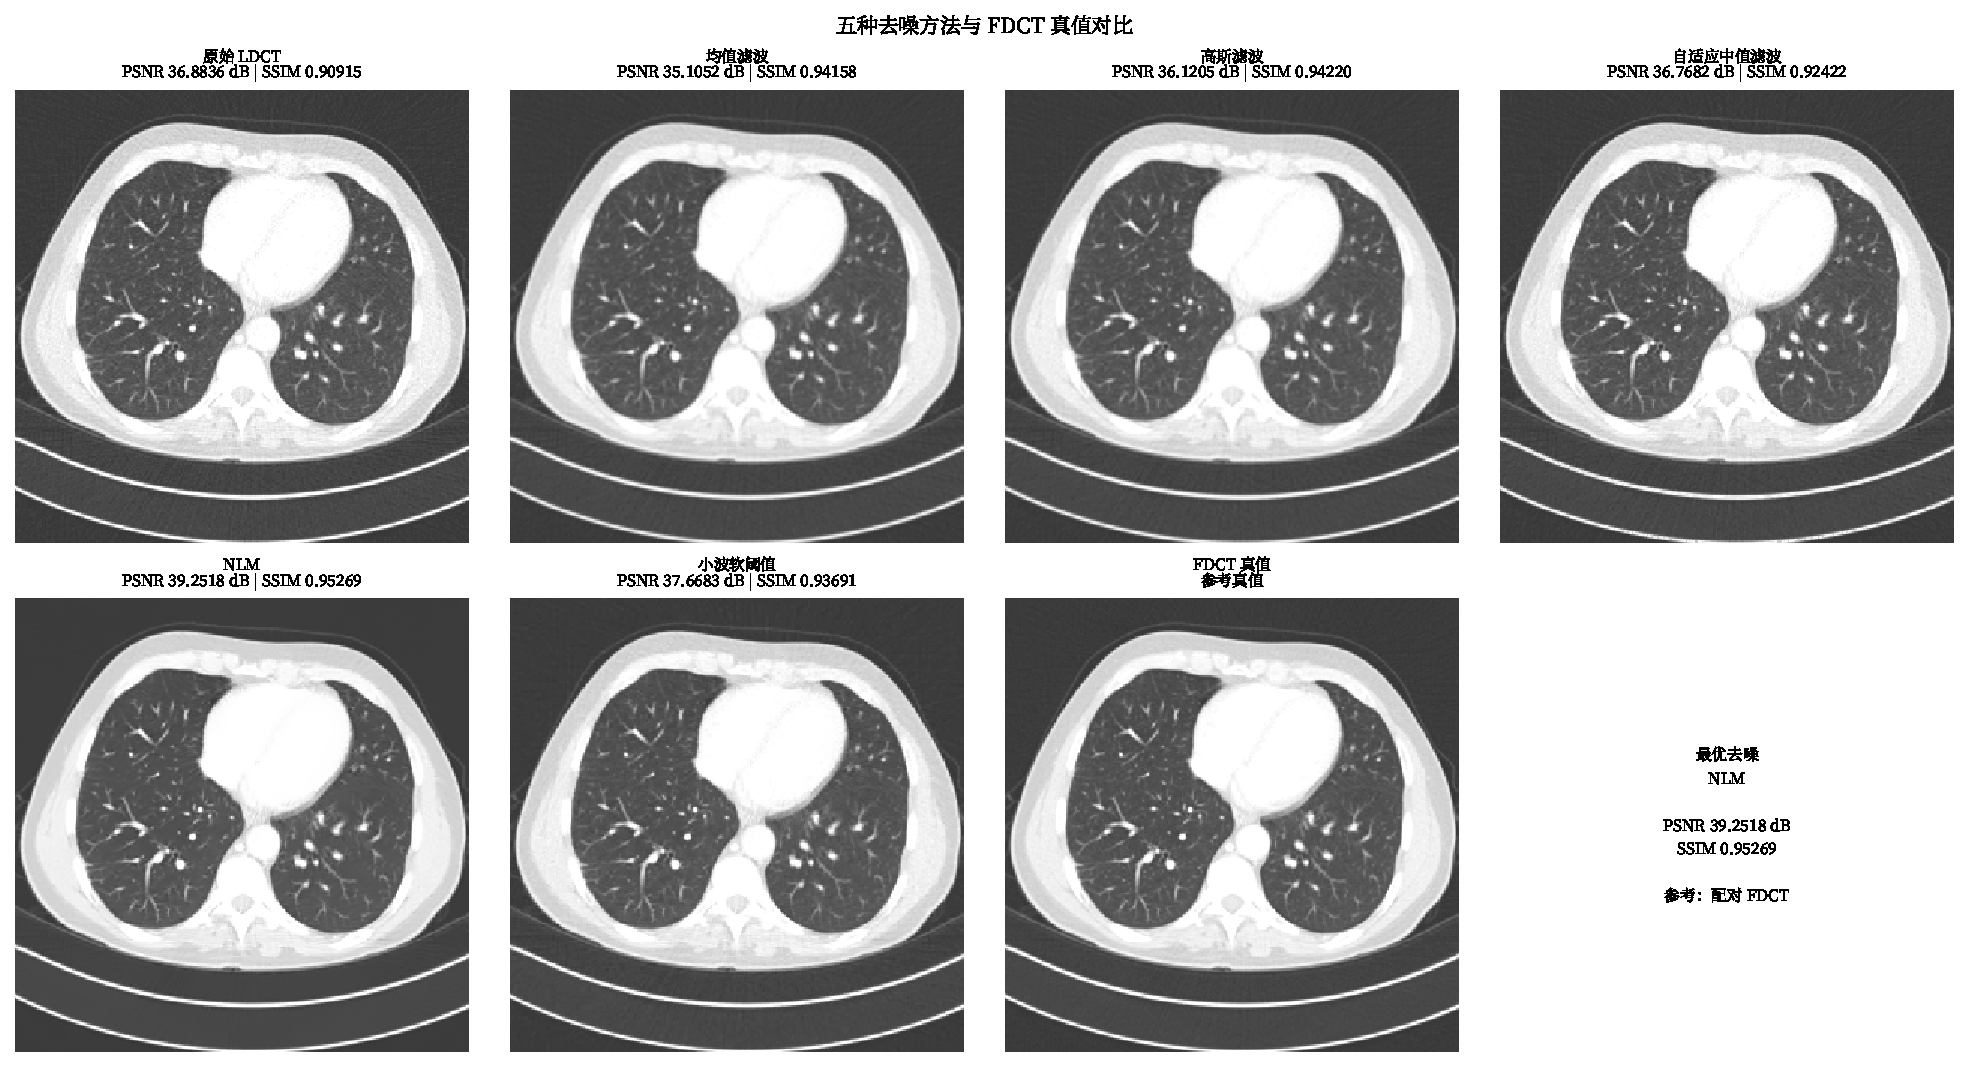
\includegraphics[width=0.95\textwidth]{comparison_denoising.pdf}
\caption{原始 LDCT、五种去噪结果与 FDCT 对比}
\label{fig:denoising}
\end{figure}

\subsection{超分辨率重建结果}

如表~\ref{tab:sr} 所示，在 NLM 去噪的基础下，三种插值方式中双三次插值的结果最优。

\begin{table}[!ht]
\centering
\caption{三种插值方法重建指标（参考图像为降采样前的 NLM 图像）}
\label{tab:sr}
\begin{tabular}{lcccc}
\toprule
方法 & PSNR (dB) & SSIM & 梯度边缘 MAE & 梯度相关系数 \\
\midrule
最近邻 & 24.665 & 0.84879 & 33.539 & 0.6647 \\
双线性 & 26.270 & 0.86476 & 27.400 & 0.8140 \\
双三次 & \textbf{28.005} & \textbf{0.88673} & \textbf{25.157} & \textbf{0.8437} \\
\bottomrule
\end{tabular}
\end{table}

如表~\ref{tab:sr} 所示，最近邻插值的 PSNR、SSIM 和梯度相关系数在三种方法中均为最低，边缘误差也最大，说明其重建效果较差。双线性插值能够明显减少最近邻插值产生的锯齿，但\added{局部细小结构边缘}仍较为模糊。相比之下，双三次插值的 PSNR（28.005 dB）和 SSIM（0.88673）均最高，梯度边缘 MAE 最低（25.157），梯度相关系数最高（0.8437），其重建边缘与降采样前的 NLM 参考图像最接近。

三种方法的综合效果排序为：双三次插值 $>$ 双线性插值 $>$ 最近邻插值。双三次插值在边缘连续性、细节保持和定量指标之间取得了最好的平衡，在本实验设置下表现最佳。

需要注意，双三次插值仍然只是根据已有像素进行估计。它可以改善显示的平滑性和视觉连续性，但不能恢复在 $128\times128$ 降采样过程中丢失的真实高频医学信息。图~\ref{fig:sr} 给出 NLM、三种插值重建与 FDCT 的并排对比。

\begin{figure}[!ht]
\centering
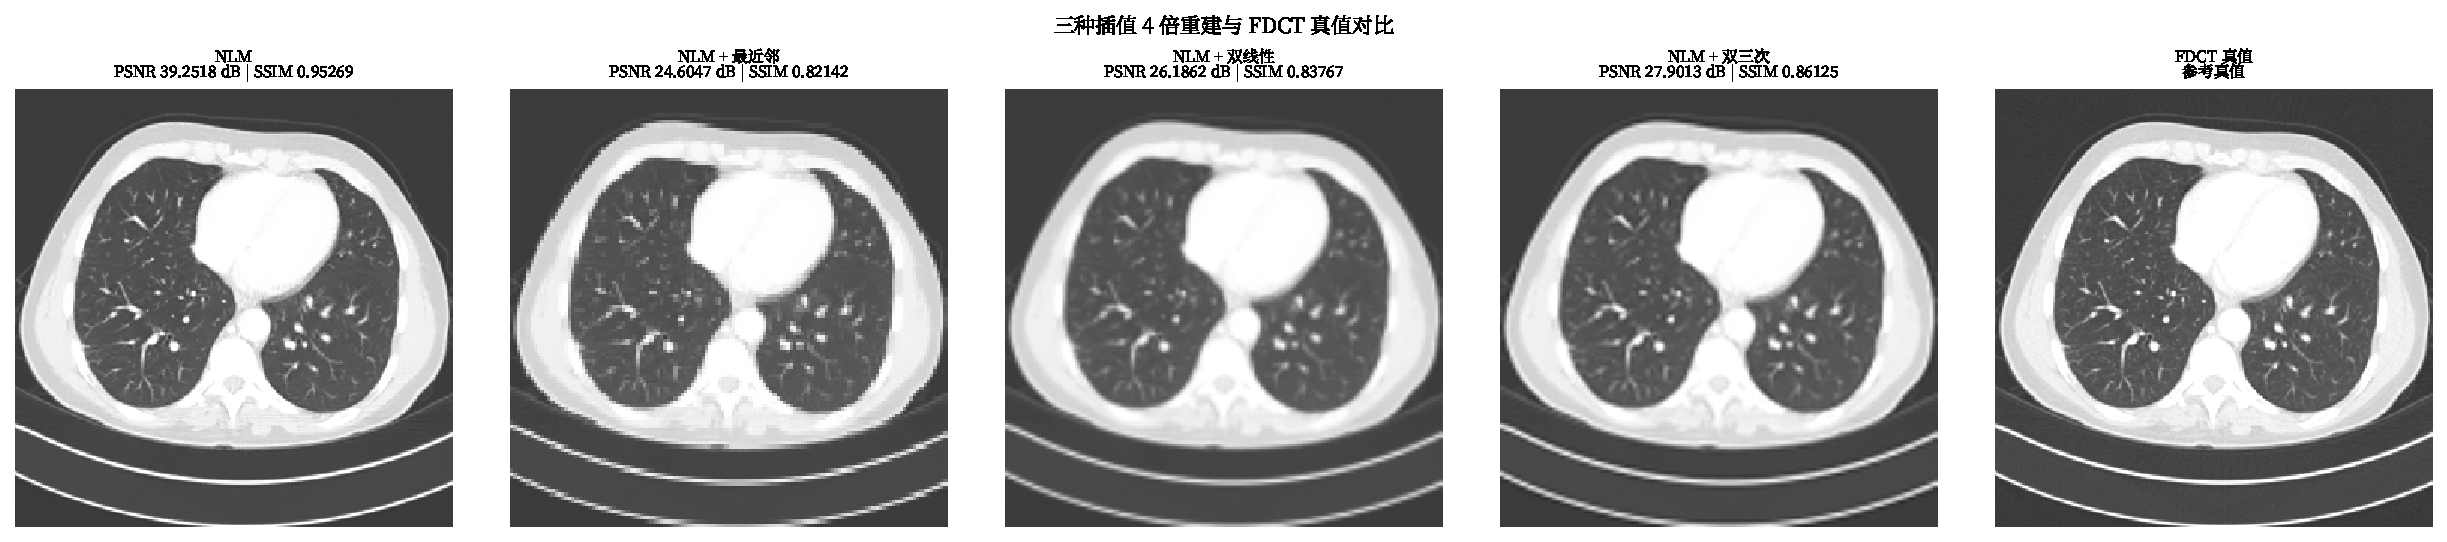
\includegraphics[width=0.95\textwidth]{comparison_sr.pdf}
\caption{NLM、三种插值重建与 FDCT 对比}
\label{fig:sr}
\end{figure}

\subsection{降噪与超分的顺序影响}

为分析降噪与超分的先后顺序是否影响最终效果，设计两组方案：

\begin{itemize}
\item 方案 A：先降噪，后超分；
\item 方案 B：先超分，后降噪。
\end{itemize}

\added{两种流程使用数值相同的 NLM 参数（\(h=4\)，模板窗口 7，搜索窗口 21）和双三次插值，仅改变执行顺序；由于处理尺寸不同，相同像素窗口对应的空间范围仍有差异，结果仅代表本次参数设置。参考图像为双三次插值放大到 \(2048\times2048\) 的 FDCT，结果如表~\ref{tab:order}。}

\begin{table}[!ht]
\centering
\caption{降噪与超分顺序影响对比}
\label{tab:order}
\begin{tabular}{ccc}
\toprule
方案 & PSNR (dB) & SSIM \\
\midrule
A 先降噪后超分 & 39.22 & 0.9693 \\
B 先超分后降噪 & 38.45 & 0.9639 \\
\bottomrule
\end{tabular}
\end{table}

如表~\ref{tab:order} 所示，先降噪再超分得到的结果优于先超分后降噪，其 PSNR 提高了 0.77 dB，SSIM 提高了 0.0054。推测是由于降噪在原始分辨率上进行时，噪声能在放大之前被抑制。若先超分，噪声会被插值放大到更大尺度，再去噪时容易把噪声与真实边缘一起平滑，导致细节损失。因此，先降噪后超分在本实验中结果更优。

\subsection{传统插值超分的固有局限}

尽管双三次插值在三种方法中综合最优，但从实验结果来看，传统插值超分存在一定局限：

\begin{enumerate}
\item 无法生成真实高频细节。传统插值主要利用已有像素估计放大后的像素值，能够改善图像的平滑性和连续性，但不能恢复原始图像中已丢失的信息。
\item 边缘细节容易受到平滑影响。插值主要根据邻域像素进行估计，对于\added{组织轮廓等局部边缘结构}，放大过程中可能出现一定程度的平滑。
\item 超分后的指标提升有限，且受到 GT 构造方式的影响。LDCT 原始 PSNR 为 36.884 dB，NLM 去噪后为 39.252 dB。而在以 FDCT 为 GT 的超分评价中，NLM+双三次超分后 PSNR 为 27.901 dB，低于 NLM 去噪本身。这说明在当前实验设置下，插值并未带来真实细节恢复，反而使重建结果与 FDCT 之间的差异增大。
\item 不能替代迭代重建或学习方法。传统插值属于后处理，无法恢复投影域丢失的信息。\added{后续可在相同数据与评价条件下比较迭代重建等方法，并扩展至更多患者和切片，以检验结论的适用范围}\redcite{yu2009dose,mccollough2017dataset}。
\end{enumerate}

\subsection{综合方案选择}

综合以上结果：

\begin{itemize}
\item 去噪方法中，NLM 最优（PSNR=39.252 dB，SSIM=0.95269）；
\item 插值方法中，双三次最优；
\item 顺序上，先降噪后超分优于先超分后降噪。
\end{itemize}

综合以上实验结果，“先 NLM 去噪、后双三次插值” 为本实验条件下的推荐处理流程。需要注意的是，在以 FDCT 为参考的最终评价中，双三次插值并未在客观指标上带来明显的进一步提升，因此该流程的优势主要体现在噪声抑制以及图像尺寸和视觉连续性的改善，而非高频医学细节的恢复。图~\ref{fig:all} 给出 LDCT、NLM、NLM+双三次与 FDCT 的并排对比。

\begin{figure}[!ht]
\centering
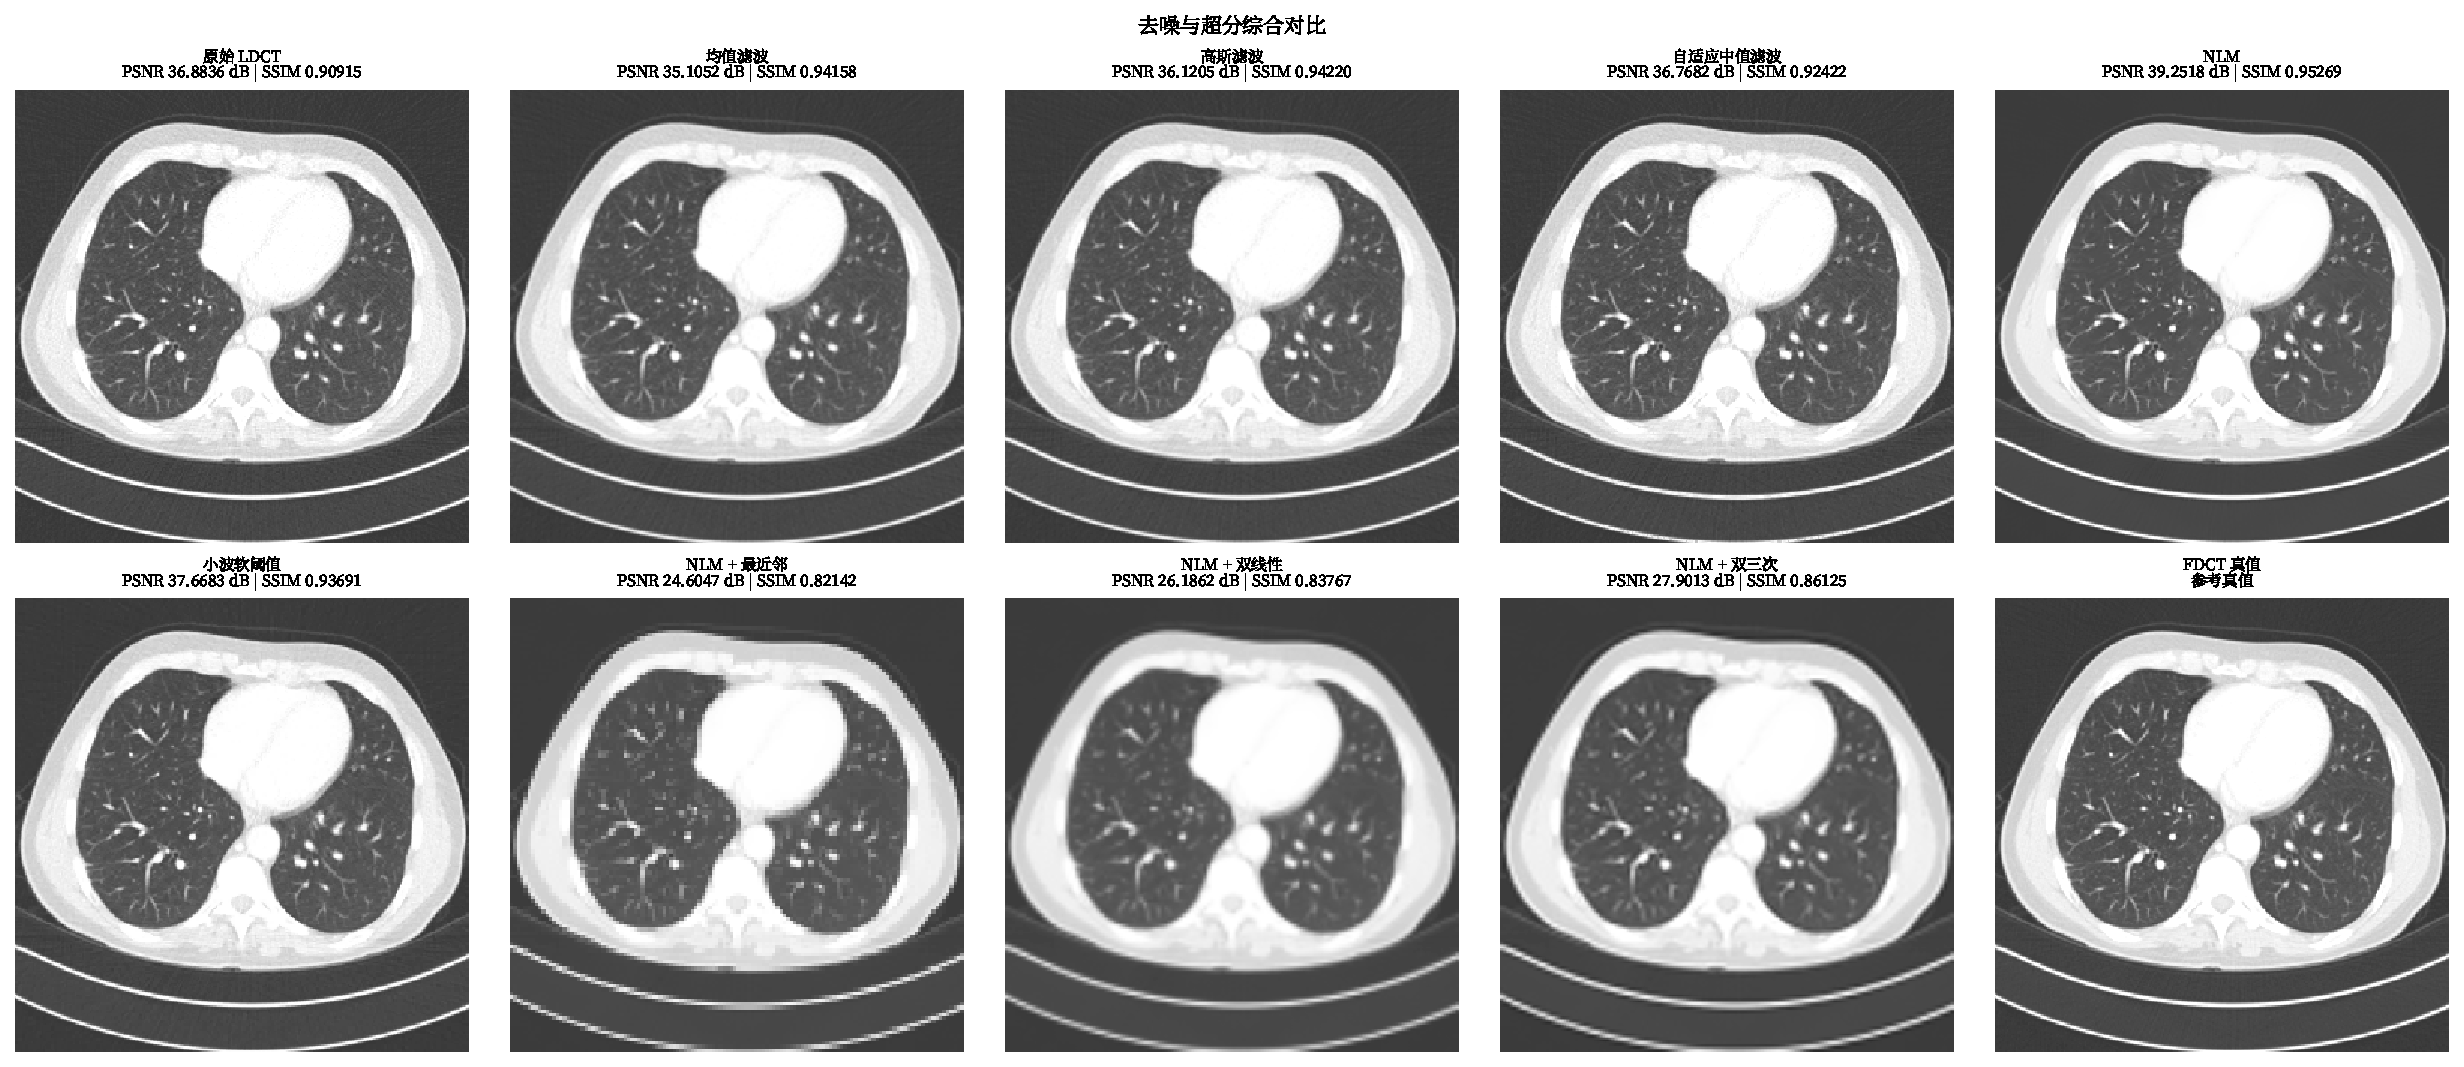
\includegraphics[width=0.95\textwidth]{comparison_all.pdf}
\caption{LDCT、NLM、NLM+双三次与 FDCT 对比}
\label{fig:all}
\end{figure}

\section{\heiti 结论}
%5 结论概括本次实验中表现较好的方法、处理顺序的影响，以及传统插值无法恢复真实缺失高频细节的限制。结论限定在实际测试数据范围内。
本文基于 AAPM2016 Mayo LDCT 数据集中的 L067 配对切片，使用纯传统图像处理方法完成了低剂量 CT 的去噪与超分辨率重建，并以全剂量 FDCT 为 Ground Truth 进行定性与定量评价。

主要结论如下：

\begin{enumerate}
\item 去噪方面：在均值滤波、高斯滤波、自适应中值滤波、NLM 和小波软阈值五种方法中，NLM 综合指标最优，其 PSNR 为 39.252 dB，SSIM 为 0.95269。与原始 LDCT 相比，PSNR 提高 2.368 dB，SSIM 提高 0.04353。
\item 超分方面：在最近邻、双线性和双三次三种插值中，双三次插值综合效果最好。在以降采样前 NLM 图像为参考的 4 倍插值实验中，双三次插值取得最高 PSNR（28.005 dB）和 SSIM（0.88673）。
\item 顺序方面：先降噪后超分优于先超分后降噪。方案 A（先降噪后超分） 的 PSNR 为 39.22 dB，SSIM 为 0.9693。方案 B（先超分后降噪） 的 PSNR 为 38.45 dB，SSIM 为 0.9639。方案 A 比方案 B 的 PSNR 高 0.77 dB，SSIM 高 0.0054。
\item 推荐方案：实验结果得出，采用 NLM 进行去噪、再使用双三次插值进行 4 倍重建的方案应为本文实验的最终推荐方案。
\item 固有局限：传统插值超分只能改善显示的平滑性和视觉连续性，无法生成真实高频医学信息。双三次插值同样存在此局限。
\item 展望：\added{后续可扩展测试患者和切片，并在相同评价条件下比较其他重建与去噪方法。}本文实验限定采用传统图像处理方法。
\end{enumerate}

本文实验仅基于 L067 的一张严格配对切片，结果可以验证代码和比较该切片上的算法，不能直接代表全部患者，也未把该切片宣称为已由医生确认的肺结节切片。

% References and appendices added in red for review.
\clearpage
\begingroup
\color{black}
\hyphenpenalty=500\relax
\section*{\heiti 参考文献}
\zihao{5-}
\bibliographystyle{gbt7714-numerical}
\bibliography{ref}
\endgroup

\clearpage
\appendix
\begingroup
\color{black}
\linespread{1.0}\selectfont
\zihao{5-}
\hyphenpenalty=0\relax
\exhyphenpenalty=0\relax
\renewcommand{\theFancyVerbLine}{\textcolor{black}{\scriptsize\arabic{FancyVerbLine}}}
\fvset{fontsize=\fontsize{8}{10}\selectfont,
  formatcom=\color{black},numbers=left,numbersep=6pt,
  xleftmargin=2em,tabsize=4,breaklines=true,breakanywhere=true,
  breakautoindent=true,breakindent=1em,
  breaksymbolleft={},breaksymbolright={}}
% Appendix contains the complete existing code only.
\section*{\heiti 附录 实验代码}
\subsection*{任务一：\texttt{task1/main.py}}
\VerbatimInput{appendix_code/task1/main.py}
\clearpage
\subsection*{任务二：\texttt{task2/denoise\_dicom.py}}
\VerbatimInput{appendix_code/task2/denoise_dicom.py}
\clearpage
\subsection*{任务三：\texttt{task3/main.py}}
\VerbatimInput{appendix_code/task3/main.py}
\clearpage
\subsection*{任务四：\texttt{task4/main.py}}
\VerbatimInput{appendix_code/task4/main.py}
\clearpage
\subsection*{任务五：\texttt{task5/task5-1.py}}
\VerbatimInput{appendix_code/task5/task5-1.py}

\endgroup

\end{document}

